\chapter{Current state of Kdyby}

To be able to lay out the roadmap, first we have to know the current state of each Kdyby package, the original purpose and the current requirements. We will only review those packages that actually made it to production and at least one usable version was released.

I have created few \gls{gh} repositories as a reminder for me to start working on some other web application development problems. I did start to work on some of them, for example on DoctrineForms, but it was never officially released. We will not discuss these incomplete packages in this thesis.

\section{State of the project}

The most relevant problem is compatibility with new versions of libraries that Kdyby integrates. Current version of \gls{nette} is 2.4 and the 3.0 is being developed, but some of Kdyby packages support only \gls{nette} 2.1 or older.

The other problems appear only when you interact with the source code which is still really important for me as a maintainer and for the contributors. Good maintainable code attracts more programmers to use it and contribute. There is no coding standard being enforced automatically on any package and no static analysis tool is checking the code. On the other hand almost all of the packages have unit and integration tests and linter checking the code for multiple versions of PHP.

\begin{figure} \label{fig:php:supported-versions}
  \centering
    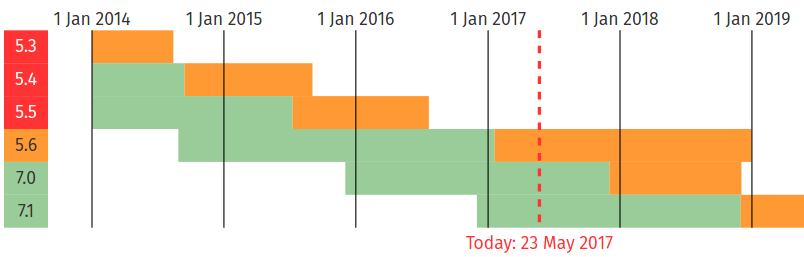
\includegraphics[width=1\textwidth]{src/assets/php-supported-versions.png}
  \caption{Supported PHP Versions. Green is active support, orange is security fixes only. Up-to-date version is at \url{https://secure.php.net/supported-versions.php}}
\end{figure}

Most of the packages are compatible with PHP 5.4, but \fnurl{PHP 5.4 had end of life at \printdate{2015-09-03}}{https://secure.php.net/eol.php} and is no longer supported by PHP developers.

PHP 5.5 had end of life at \printdate{2016-06-21} and PHP 5.6 is currently in the phase of security fixes only and will have end of life at \printdate{2018-12-31}. As you can see on the graph~\ref{fig:php:supported-versions}, everyone should be migrating to PHP 7.0 by now. But developer has to consider what PHP versions the libraries support, upgrade them first and then migrate the application.

Most of the packages are compatible with \gls{hhvm} but \gls{nette} has dropped the compatibility making it impossible to maintain.

\section{State of each package}

This section reviews each package separately, considers the original purpose and sums up the current state.

\hiddensubsection{Doctrine} \label{sec:state:doctrine}

\gls{kDoctrine} is an integration of \gls{doctrine} into \gls{nette}. But it has cumulated a lot of responsibilities that do not belong to it

\gls{doctrine} itself is separated into several packages, mainly \fnurl{doctrine/orm}{https://github.com/doctrine/doctrine2}, \fnurl{doctrine/common}{https://github.com/doctrine/common}, \fnurl{doctrine/annotations}{https://github.com/doctrine/annotations}, \fnurl{doctrine/cache}{https://github.com/doctrine/cache} and \fnurl{doctrine/collections}{https://github.com/doctrine/collections}. What started as a monolith integration in Kdyby, got separated into \gls{kEvents}~\ref{sec:state:events}, \gls{kConsole}~\ref{sec:state:console}, \gls{kAnnotations}~\ref{sec:state:annotations} and \gls{kDoctrineCache}~\ref{sec:state:doctrine-cache} for reusability.

I have already started extracting few of them in the past, for example an entity prototyping tool~\ref{sec:state:doctrine-magic-accessors}, collection utilities~\ref{sec:state:doctrine-collections-lazy}, \ref{sec:state:doctrine-collections-readonly} and helper for loading big SQL scripts into the database.

There is a big issue \fnurl{Chop up the package}{https://github.com/Kdyby/Doctrine/issues/238} that discusses what other parts should be separated and dropped completely.

New versions of \gls{nette} and \gls{doctrine} were released and completely new versions are being prepared which the integration cannot be currently used with.

\hiddensubsection{Console} \label{sec:state:console}

\gls{kConsole} is an integration of \gls{sfConsole} that allows for writing interactive CLI applications. \gls{kDoctrine} depends on this package and is the reason this package exists.

There are tasks that are better suited for console interaction, than a web interface. Among others, \gls{doctrine} has tools for generating a database schema from the entities metadata and there is a console command for it that is written using \gls{sfConsole}.

The library is solving several problems with CLI applications in \gls{nette} that are no longer relevant or have to be refactored. One of the issues is that it introduced level of abstraction above \gls{nette} Front Controller to solve generating URLs in CLI. \gls{nette} was refactored to account for this problem and this part of \gls{kConsole} is now causing more problems than it solves.

\hiddensubsection{Events} \label{sec:state:events}

\gls{kEvents} provides an event dispatcher implementation for \gls{nette}.

It started as an integration of \gls{doctrine} EventManager, but then it evolved into a standalone system with support for lazy initialization of listeners and it also contains a naive bridge for \gls{sfEventDispatcher}.

Creating such interchangeable eventing system turned out to be a mistake. The bridging of the subscriber classes is fragile and requires a lot of compromises from the programmer. It is also a maintenance hell. The systems should have stayed separate.

\hiddensubsection{Annotations} \label{sec:state:annotations}

\gls{kAnnotations} is a simple integration of doctrine/annotations into \gls{nette}. It was created solely for the purposes of \gls{kDoctrine}, but it can be used in any \gls{nette} application that requires annotations for some functionality.

The problem the doctrine/annotations solves is that PHP doesn't have native annotations. But Doctrine simulates them using PHPDoc. The example code~\ref{fig:php:annotations-example} illustrates usage of \gls{doctrine} annotations on entities. \gls{doctrine} can read this as metadata and also generate SQL schema for relational databases.

\begin{figure} \label{fig:php:annotations-example}
\begin{lstlisting}
/**
 * @Entity
 */
class Comment
{
    /**
     * @Id
     * @GeneratedValue
     * @Column(type="string")
     */
    private $id;

    /**
     * @ManyToOne(
     *     targetEntity="User",
     *     inversedBy="comments"
     * )
     */
    private $author;
}
\end{lstlisting}
\caption{Example of PHPDoc with annotations that the doctrine/annotations can parse from source code.}
\end{figure}

\gls{kAnnotations} is almost up-to-date, because it is very simple and the old version for \gls{nette} still works well for the current versions.

\hiddensubsection{DoctrineCache} \label{sec:state:doctrine-cache}

\gls{kDoctrineCache} integrates doctrine/cache that is used by doctrine/annotations and doctrine/orm to store metadata, results of various parsers and even query results.

This package has no \gls{nette} CompilerExtension, but only a helper class that configures the caching services and is used by CompilerExtensions in \gls{kAnnotations} and \gls{kDoctrine}. As such, there are only few minor problems and inefficiencies that have to be fixed to work perfectly with current \gls{nette} and Doctrine.

\hiddensubsection{DoctrineMagicAccessors} \label{sec:state:doctrine-magic-accessors}

\gls{kDoctrineMagicAccessors} is a prototyping tool for writing less code in entities. It allows to not write getters and setters for entity properties.

In \gls{doctrine} there is an entity lazy--loading feature that in order to work the entity cannot have any public properties, only protected or private. Which means that to be able to access the properties the developer has to define methods on the entity. This is completely correct, but when prototyping an application, it might not be obvious what methods will be required and what data they should allow to be written into the entity. This package aims to solve that, by allowing not to write the accessor methods, because it makes them available dynamically.

It was extracted from \gls{kDoctrine} and currently only exists to ease migrating away from this technique. The problem this package solves is still valid because manually writing getters and setters in PHP is tedious and error-prone, but the way the package does it creates more problems than it solves. Having the manually written accessors checked by static-analysis tool like \gls{phpstan} and unit tested is a better option.

\hiddensubsection{DoctrineCollectionsReadonly} \label{sec:state:doctrine-collections-readonly}

Entities in \gls{doctrine} can have associations in them. For example a cart entity might contain collection of order items. Adding an order item to the cart might be done using a \lstinline{addOrderItem} method or through the collection directly as shown in~\ref{fig:collections-readonly:example}.

When we try to modify the collection outside of the entity that owns it, we are breaking the encapsulation of that entity - it no longer has the control over what is in the collection. Therefore allowing the programmer to access the mutable collection directly is a bad practice.

\begin{figure} \label{fig:collections-readonly:example}
\begin{lstlisting}
class Cart
{
  private $orderItems;

  public function __construct() {
    $this->orderItems = new ArrayCollection();
  }

  public function addOrderItem(
    OrderItem $orderItem
  ): void {
    $this->orderItems->add($orderItem);
  }

  public function getOrderItems(): Collection {
    return $this->orderItems;
  }
}

$cart = new Cart();

// modifying the collection through entity API
$cart->addOrderItem(new OrderItem());

// modifying the collection outside of entity
$cart->getOrderItems()->add(new OrderItem());
\end{lstlisting}
\caption{Example of working with doctrine/collections.}
\end{figure}

The package \gls{kDoctrineCollectionsReadonly} provides a decorator for collections that disables methods for mutation of the collection, but keeps available those that only read data. This allows the entity to expose the collection, so that the programmer can use the friendly collections API, without having to worry to accidentally modify the internal state of the owning entity.

\begin{figure} \label{fig:collections-readonly:readonly}
\begin{lstlisting}
public function getOrderItems(): Collection {
  return new ReadOnlyCollectionWrapper(
    $this->orderItems
  );
}

// returns first OrderItem
$orderItem = $cart->getOrderItems()->first();

// throws exception
$cart->getOrderItems()->add(new OrderItem());
\end{lstlisting}
\caption{Example of DoctrineCollectionsReadonly in entity.}
\end{figure}

\gls{kDoctrineCollectionsReadonly} depends only on doctrine/collections which did not change drastically and there no changes required for the package to function with new versions.

\hiddensubsection{DoctrineCollectionsLazy} \label{sec:state:doctrine-collections-lazy}

\Gls{kDoctrineCollectionsLazy} package provides implementation of doctrine/collections Collection interface that accepts a generator function and evaluates it lazily, only when the items are actually accessed.

\gls{kDoctrineCollectionsLazy} depends only on doctrine/collections and therefore the situation is the same as with \gls{kDoctrineCollectionsReadonly}.

% \hiddensubsection{DoctrineDbalBatchImport} \label{sec:state:doctrine-dbal-batch-import}

% \Gls{doctrine} does not have any tool for importing a big SQL file and this package provides helpers for it. It allows iterating over huge file in a memory effective way, executing each SQL query it finds in it.

% \gls{kDoctrineDbalBatchImport} has no stable version yet, but as a former part of \gls{kDoctrine}, it has to be refactored and the stable versions released.

\hiddensubsection{Curl} \label{sec:state:curl}

PHP has a binding for the Curl library and exposes its functions to the programmer. But the API is the same as the underlying C API, which is not suited for modern \gls{oop} development. \gls{kCurl} is wrapping the Curl functions in \gls{oo} API.

There are now better and more popular packages for doing HTTP requests in PHP like \fnurl{guzzlehttp/guzzle}{https://github.com/guzzle/guzzle}. Therefore this package is now deprecated and unmaintained.

\hiddensubsection{CurlCaBundle} \label{sec:state:curl-ca-bundle}

For doing secured HTTP requests over HTTPS the client must have available the public certificates that signed the private certificates the website is using to establish the secured connections. There are hosting providers that do not regularly update the certificates in the operating system. This creates a problem that this package solves.

I have a cron job on my \gls{vps} that regularly downloads fresh certificates from Mozilla browser, extracts them to format that the Curl clients can use and then publishes them as a new version of \gls{kCurlCaBundle}.

Using this package in application means it no longer depends on outdated system certificates and they can be updated regularly with this package.

The Composer authors created their own package \fnurl{composer/ca-bundle}{https://github.com/composer/ca-bundle} that solves this problem too. And since Composer has bigger user base, it gained traction and is now de~facto a standard. Therefore \gls{kCurlCaBundle} is now deprecated. But since a lot of applications still depend on it, I am maintaining the cron job and keeping the package alive until everyone adopts composer/ca-bundle.

\hiddensubsection{Autowired} \label{sec:state:autowired}

\gls{kAutowired} was an experiment with \gls{di} in \gls{nette} presenters. \gls{nette} presenters are similar to Controllers in \gls{mvc} pattern, but have slightly different responsibilities. As such, they accept services through \gls{di} and then process the application request. Since presenters in \gls{nette} are usually part of big inheritance tree, their parents might have several dependencies that the children would have to pass through their constructors to the parents introducing what we were calling constructor hell.

\gls{kAutowired} helps with the problem by allowing to declare the dependencies in presenter properties with a special annotation. These dependencies would not have to be passed through constructor, because they are initialized lazily when they are accessed.

This works reliably, but breaks encapsulation of the presenter classes. The right solution to this problem is to have more lightweight \lstinline{UI\Presenter}, with fewer responsibilities.

The second issue \gls{kAutowired} solves is fetching \gls{ui} component factories that create the instance of the \gls{ui} component and passing them into presenter component factories that configure the \gls{ui} component for the specific use--case.

Autowiring of the factories doesn't break encapsulation of the presenter class, but it breaks the \gls{di} principle, by not exposing the direct dependencies of the presenter class, but instead it makes the presenter depend on \gls{dic} which is considered an anti--pattern.

\hiddensubsection{FormsReplicator} \label{sec:state:forms-replicator}

Forms component of \gls{nette} has a lot of capabilities, but it does not support repeating an input field, or group of them, dynamically. This means the application is very strict about what fields it accepts when a form is submitted in browser. That is generally good for security, but sometimes it is required to accept dynamic amount of fields when the form is expected to be modified on the client and the application does not know ahead how many fields will be sent by the user. \gls{kFormsReplicator} solves this by creating the form using the data the user sent.

This library worker perfectly with \gls{nette} 2.1 but the Forms component was refactored heavily since then and the assumptions this package worked on were broken. This means there are a lot of bugs when it is used with newer \gls{nette}.

\hiddensubsection{Translation} \label{sec:state:translation}

Translating the application \gls{ui} and the content itself are two very different problems. \gls{kTranslation} solves the first problem. It integrates \gls{sfTranslation} into \gls{nette}.

In the past, the \gls{sf} Bundle for integrating \gls{sfTranslation} the did contain few important parts that \gls{kTranslation} has to duplicate, but not anymore. The 3.0 version provides all required functionality and the duplication can now be removed from \gls{sfTranslation}.

\hiddensubsection{Validator} \label{sec:state:validator}

\gls{kValidator} is very thin integration of \gls{sfValidator} into \gls{nette}.

\hiddensubsection{RabbitMq} \label{sec:state:rabbit-mq}

\gls{kRabbitMq} integrates php-amqplib/php-amqplib into \gls{nette} and php-amqplib/php-amqplib is a client for RabbitMq server. \gls{kRabbitMq} provides producer classes that are used to generate messages for the RabbitMq server and consumer classes that listen for incoming messages from the RabbitMq server and processes them with user-defined logic. It depends on \gls{kConsole}, since the consumers are started as standalone processes through CLI. The php-amqplib/php-amqplib had supported old PHP versions for very long and now it is hard to change the internal design of it and \gls{kRabbitMq} hides that using abstraction.

The php-amqplib/php-amqplib changed maintainers and it has to be reviewed for new functionality that might benefit the users of \gls{kRabbitMq}. There are also important features like \fnurl{SSL connection support}{https://github.com/Kdyby/RabbitMq/issues/5} that were never implemented.

\hiddensubsection{Money} \label{sec:state:money}

PHP does not have a native Decimal type, only float. And floats cannot be used to represent money values. Libraries exist that solve this exact problem. One level of abstraction above that are money libraries that use the decimal implementations to represent the money values paired with currency.

\gls{kMoney} is meant to be simpler and have more clean architecture than other competitive implementations. It operated with cent values in integers to avoid float rounding problems.

It is now deprecated, because it was really hard to maintain and there were bugs with rounding even with the integers implementation.

\hiddensubsection{DoctrineMoney} \label{sec:state:doctrine-money}

\gls{kDoctrineMoney} integrates \gls{kMoney} into \gls{kDoctrine}. Since \gls{kMoney} was deprecated, this package is now deprecated too.

\hiddensubsection{Aop} \label{sec:state:aop}

\gls{kAop} is a custom implementation of \gls{aop} for \gls{nette} \gls{dic} component. It searches the aspect definitions, finds the services they are supposed to advice and creates proxy classes from them. In the proxy classes, it overrides the methods and applies the aspect advices.

This package was created for \gls{nette} 2.1 and \gls{nette} \gls{dic} component internals were refactored heavily since. This means the package has to be review for possible problems and updated to current libraries.

\hiddensubsection{Clock} \label{sec:state:clock}

Logic in application often depends on current time, but if you want to unit test such logic, it is a problem. \gls{kClock} solves this problem by implementing a DateTimeProvider service for \gls{nette}. The service with time sensitive logic should require the DateTimeProvider interface and every time it requires to know the current date and time it calls a \lstinline{getTime()} method on the provider. With the dependency clearly declared in constructor of the service, it can be easily mocked and unit tested.

The package works well, but it would be useful to have such functionality framework agnostic. Now the package depends on \gls{nette}.

\hiddensubsection{Redis} \label{sec:state:redis}

\gls{kRedis} integrates the \fnurl{Pecl}{https://secure.php.net/manual/en/install.pecl.intro.php} extension \fnurl{Redis}{https://pecl.php.net/package/redis} into \gls{nette}. There are three main services it provides - cache, cache journal, sessions and locking.

Redis is fast memory key-value storage and as such is a great candidate for cache storage. \gls{nette} contains \lstinline{IStorage} interface that \gls{kRedis} implements and it can be used as a drop-in replacement for the default file caching.

Journal in \gls{nette} is used for keeping track of tags assigned to cache values. This metadata can be then used to invalidate only specific keys in cache. The default journal in \gls{nette} was historically implemented using custom binary file and now is implemented as an SQLite database. The binary file implementation was limited by the format and could only store fixed amount of key and value pairs which is perfectly fine up to a certain point of application growth. Now the current solution with SQLite database does not have this problem, but still it requires a local file system to work. \gls{kRedis} implementation uses native Redis data structures to implement the journaling and can be used as a replacement, if the other implementations are not ideal for the application.

Session handler takes care of user sessions. In order to implement login functionality, web application has to assign session cookies to visitors and the session cookie value is used as key for session storage allowing the website to store information per user. The default implementation in PHP uses file system and is prone to failure with high traffic, because of its garbage collection mechanism. The default Redis PHP extension has its own session handler, but this handler does not handle locking of the sessions, which means a high chance for a race condition where older application request might rewrite data from newer application request. This is acceptable, if the application doesn't store any additional data in the session, apart from the user id. But typical \gls{nette} application stores at least flash messages in sessions and its undesirable for them to get lost.

Redis server does not have any form of native locking. It only recommends the locking algorithm \fnurl{Redlock}{https://redis.io/topics/distlock} and \gls{kRedis} implements it.
It is used for locking cache keys when the IStorage from \gls{nette} is required to block and it is also used for the custom session handler.

\gls{kRedis} contains thin abstraction over the Redis PHP extension that is probably not necessary for the caching, journal and session services.

\hiddensubsection{Monolog} \label{sec:state:monolog}

\gls{kMonolog} is an integration of \fnurl{monolog/monolog}{https://github.com/Seldaek/monolog} library that implements \gls{psr}-3 into \gls{nette}. \gls{kMonolog} handles integration with Tracy as well, making every exception passed to Monolog render with every relevant detail using Tracy BlueScreen renderer.

The integration works well even with current \gls{nette}, but has a lot of dead code for providing backwards compatibility that can be dropped when the version requirement for \gls{nette} is increased. Also the configuration structure is suboptimal. The configuration of \gls{sf} bundle for Monolog is better and \gls{nette} would benefit from having the same structure.

\hiddensubsection{ElasticSearch} \label{sec:state:elastic-search}

There are two main client packages for \gls{elastic} - \fnurl{ruflin/elastica}{https://github.com/ruflin/Elastica} and \fnurl{elasticsearch/elasticsearch}{https://github.com/elastic/elasticsearch-php}. \gls{kElasticSearch} integrates ruflin/elastica into \gls{nette}. The 1.* versions of elasticsearch/elasticsearch were tightly coupled with 3rd party \gls{dic} which lead to choosing the ruflin/elastica package. The main benefit of this package is the Tracy panel that prints executed queries which allows for easier debugging.

There are several new major versions of both libraries. The Tracy panel and the bridging has to be review for bugs and possible improvements.

\hiddensubsection{DoctrineSearch} \label{sec:state:doctrine-search}

\gls{kDoctrineSearch} integrates \fnurl{doctrine/search}{https://github.com/doctrine/search} into \gls{nette} and extends it for a specific use--case we required at Rohlik.

\hiddensubsection{Geocoder} \label{sec:state:geocoder}

\gls{kGeocoder} extends \fnurl{willdurand/geocoder}{https://github.com/geocoder-php/Geocoder} with custom geo\-co\-de\-r provider for \fnurl{Seznam maps}{https://api.mapy.cz/}, logging capabilities and mechanism for sorting the results.

The geo\-co\-de\-r declares a common interface for communication with maps data API providers. There are two main tasks - geocoding and reverse geocoding. Geocoding is a search in maps data for given string that returns list of addresses with GPS coordinates that correspond to the search query. Reverse geocoding takes a GPS coordinate and returns the address that corresponds to it. A geo\-co\-de\-r provider is implementation of the common geocoding interface for the specific maps data provider.

The package now solves 4 different problems and is tightly coupled with old versions of \gls{nette}, but is well covered with unit tests.

\hiddensubsection{CsobPaymentGateway} \label{sec:state:csob-payment-gateway}

The czech ČSOB bank has created its own payment gateway for paying with debit and credit cards that can be used with any web or mobile application. \gls{kCsobPaymentGateway} is a client that wraps the API communication in \gls{oo} abstraction. The main concerns are security and simplicity of use, since this library is part of the most critical application infrastructure - the payment process.

At the same month this library was published a competitive package \fnurl{slevomat/csob-gateway}{https://github.com/slevomat/csob-gateway} was released. It is impossible to support package this critical without having it in production and being able to monitor it. Since I have left the company we needed this integration for, I did not have a chance to deploy the package to any new project that I would maintain and the new versions and features of the ČSOB payment gateway are not implemented. This makes the library dangerous to use which lead to a \fnurl{search for new maintainer of \gls{kCsobPaymentGateway}}{https://github.com/Kdyby/CsobPaymentGateway/issues/25}.

\hiddensubsection{CsobPaygateNette} \label{sec:state:csob-paygate-nette}

\gls{kCsobPaygateNette} integrates \gls{kCsobPaymentGateway} into \gls{nette} and provides a \gls{ui} component for easier implementation of payment handling logic.

\hiddensubsection{Wkhtmltopdf} \label{sec:state:wkhtmltopdf}

\fnurl{Wkhtmltopdf}{https://wkhtmltopdf.org/} is, among others, a PDF generator. It has CLI interface that accepts a HTML file, set of options and generates a PDF. \gls{kWkhtmltopdf} is a \gls{oo} abstraction of the CLI for \gls{nette}. It contains a lot of custom solutions for the subproblems that are not easy to maintain. There are also several new versions of the tool.

\hiddensubsection{FakeSession} \label{sec:state:fake-session}

\gls{nette} is first of all \gls{mvc} framework which means most applications written in it depend on PHP sessions heavily. Having an abstraction that disables the mechanism but does not break application in the context of a single request is useful for writing integration tests that would otherwise interfere with each other and making sure REST API does not leak any cookies even with programmer mistake would cause it do so. \gls{kFakeSession} replaces the default session mechanism in \gls{nette} with custom one that operates only in the memory of the current PHP process.

It is working well even with current versions of \gls{nette} but it has only few integration tests and no unit tests.

\hiddensubsection{RequestStack} \label{sec:state:request-stack}

\gls{nette} is designed to operate in the context of a single HTTP request that maps on a single application request. Therefore it has \lstinline{Http\Request} object as a shared service that any service registered into \gls{dic} can request and depend on. If one would require to handle two separate application requests, references of \lstinline{Http\Request} object from the first request would already be permanently bound to all the services in \gls{dic}. \gls{kRequestStack} replaces the service implementation of a value object for a container of the \lstinline{Http\Request} that delegates the method calls to it which means all the services have references for the \lstinline{RequestStack} service that never changes and more request can be handled by simply switching the \lstinline{Http\Request} reference inside the container. A perfect solution would be to redesign \gls{nette} internals to handle this problem correctly, but that would be a big architecture challenge to not break the compatibility with almost every application.

\gls{kRequestStack} has very few unit tests but is very simple. There have been changes in the way the related services are configured in \gls{nette} and the integration requires a small refactoring to account for this.

\hiddensubsection{StrictObjects} \label{sec:state:strict-objects}

PHP itself is very tolerant about object properties. It is possible to assign value to a property that is not defined on the class of the object and it works correctly. This dynamic behavior might be useful, but has no place in serious applications since it introduces a big potential for errors. The more strict the application is about types, the safer it usually is. \gls{kStrictObjects} introduces a trait which is glorified mechanism for copy and paste of code between objects that fixes this behavior. PHP allows classes to implement magic methods that are called when undefined property or method is accessed. The \gls{kStrictObjects} trait defines them and throws exception any time you try to access undefined method or property of the class.

The package is stable, does not depend on \gls{nette} and the only problem it has at this moment is no support for PHP 7.1.

\hiddensubsection{Facebook} \label{sec:state:facebook}

With applications that need to interact with Facebook there are two main use--cases - Facebook OAuth login and advertisement data manipulation. Both require secure communication with the \gls{fbApi}. \gls{kFacebook} supports the OAuth 2 login mechanism of Facebook and provides a client for the \gls{fbApi} communication.

Facebook keeps releasing new version of their API that keeps breaking backwards compatibility which results in a lot of maintenance work of \gls{kFacebook}. But the package did not receive enough attention and the last supported version of \gls{fbApi} is \lstinline{v2.3} which is supported only until \printdate{2017-08-07} and as of writing this the current \fnurl{version of \gls{fbApi}}{https://developers.facebook.com/docs/apps/changelog} is \lstinline{v2.9}.

\hiddensubsection{Google} \label{sec:state:google}

\gls{kGoogle} is an integration of \fnurl{google/apiclient}{https://github.com/google/google-api-php-client} which aims to solve primarily OAuth 2 login functionality for \gls{nette}. It was written with old PHP 5.3, users report it cannot be even easily installed.

\hiddensubsection{\gls{gh}} \label{sec:state:github}

\gls{kGithub} is a custom implementation of a \gls{gh} API client and its integration into \gls{nette}. It enables secure authentication when its \gls{ui} component is used.

\hiddensubsection{BootstrapFormRenderer} \label{sec:state:bootstrap-form-renderer}

The CSS framework \fnurl{Twitter Bootstrap}{http://getbootstrap.com/} has a specific markup of HTML forms that is very different from what \gls{nette} Forms component generates by default. This package implements a custom Forms renderer that enables simpler markup and often completely automatic rendering of most forms a typical application might have. The package was relevant for Twitter Bootstrap 2.2 and Nette 2.1. New versions of \gls{nette} have more features enabling them to be configured to render the required markup by default instead of having to replace the renderer. The package is currently abandoned and unmaintained.

\hiddensubsection{PayPalExpress} \label{sec:state:paypal-express}

PayPal is popular payment platform and \gls{kPayPalExpress} provided a custom API client and its integration into \gls{nette}. Now is deprecated because I had no use for it in any production application and no new maintainer was found which means its dangerous to invite other people to use it.

\hiddensubsection{PresentersLocator} \label{sec:state:presenters-locator}

There is a \lstinline{PresenterFactory} in \gls{nette} that is responsible for mapping the application request details to appropriate presenter class and then creating instance of it. In current versions of \gls{nette} the \lstinline{PresenterFactory} delegates the creation of the instance to the \gls{dic} but it was not doing it in older versions of \gls{nette}. \gls{kPresentersLocator} is automatically discovering presenter classes in the application and registering them as services in compile--time of the \gls{dic}. Since \gls{nette} currently solves this problem without the need for this extension, it was deprecated.
